\documentclass[tikz]{standalone}



\begin{document}
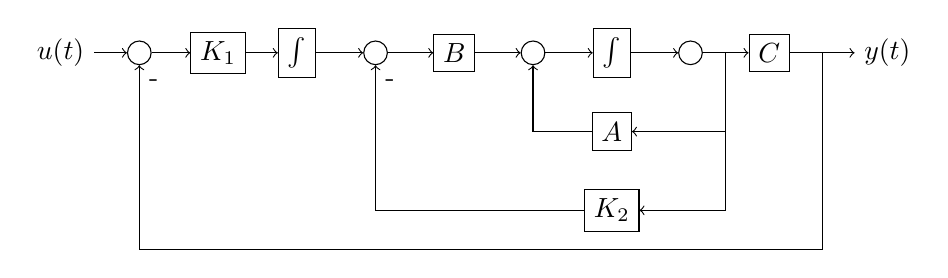
\begin{tikzpicture}[x=10mm]
\coordinate (A) at (0,0);
\coordinate (B) at (1,0);
\coordinate (C) at (2,0);
\coordinate (D) at (3,0);
\coordinate (E) at (4,0);
\coordinate (F) at (5,0);
\coordinate (G) at (6,0);
\coordinate (H) at (7,0);
\coordinate (I) at (8,0);
\coordinate (J) at (9,0);
\coordinate (K) at (10.5,0);
\coordinate (L) at (7, -1);
\coordinate (M) at (7,-2);


\node (A1) at (A) {$u(t)$};
\node[circle,draw,inner sep=0pt,minimum size=3mm] (B1) at (B) {};
\node[rectangle,draw] (C1) at (C) {$K_1$};
\node[rectangle,draw] (D1) at (D) {$\int$};
\node[circle,draw,inner sep=0pt,minimum size=3mm] (E1) at (E) {};
\node[rectangle,draw] (F1) at (F) {$B$};
\node[circle,draw,inner sep=0pt,minimum size=3mm] (G1) at (G) {};
\node[rectangle,draw] (H1) at (H) {$\int$};
\node[circle,draw,inner sep=0pt,minimum size=3mm] (I1) at (I) {};
\node[rectangle,draw] (J1) at (J) {$C$};
\node (K1) at (K) {$y(t)$};
\node[rectangle,draw] (L1) at (L) {$A$};
\node[rectangle,draw] (M1) at (M) {$K_2$};

\draw[->] (A1) -- (B1);
\draw[->] (B1) -- (C1);
\draw[->] (C1) -- (D1);
\draw[->] (D1) -- (E1);
\draw[->] (E1) -- (F1);
\draw[->] (F1) -- (G1);
\draw[->] (G1) -- (H1);
\draw[->] (H1) -- (I1);
\draw[->] (I1) -- (J1) coordinate[midway] (I2);
\draw[->] (J1) -- (K1) coordinate[midway] (K2);
\draw[->] (I2) |- (L1) coordinate[midway] (I3);
\draw[->] (L1) -| (G1);
\draw[->] (I3) |- (M1);
\draw[->] (M1) -| (E1) node[pos=1,anchor=north west] {-};
\draw[->] (K2) --++ (0,-2.5) -| (B1) node[pos=1,anchor=north west] {-};


\end{tikzpicture}
\end{document}